\documentclass[areasetadvanced]{scrartcl}

\usepackage[utf8]{inputenc}
\usepackage[T2A]{fontenc}
\usepackage[english,russian]{babel}

\usepackage[footskip=1cm,left=25mm, right=15mm, top=20mm, bottom=20mm]{geometry}
\usepackage{setspace}
\usepackage{amsmath, amssymb}  % Объединено в одну строку
\usepackage{graphicx}
\usepackage{tikz}
\usetikzlibrary{arrows.meta}
\usepackage{float}
\usepackage{dashrule}
\usepackage{fancyhdr} % оформление отчёта
\usepackage{hyperref} % оформление отчёта
\usepackage{parskip}
\usepackage{textcomp, enumitem}
\usepackage{indentfirst}
\usepackage{graphicx}
\usepackage{algorithm}
\usepackage{algpseudocode}
\usepackage{array}  % Для использования команды m{}
\usepackage{geometry}
\usepackage{afterpage}
\usepackage{minted}
\setcounter{secnumdepth}{3}  % Включает нумерацию для subsubsection
\setcounter{tocdepth}{3}     % Включает subsubsection в содержание
\usepackage{listings} % Если используете listings
\setlength{\parindent}{1.25cm}
\tikzstyle{block} = [rectangle, rounded corners, minimum width=3cm, minimum height=1cm, text centered, draw=black, fill=lightgray]

\setkomafont{sectioning}{\normalfont\bfseries} % для заголовков разделов и подразделов
\setkomafont{section}{\normalfont\Large\bfseries}
\setkomafont{subsection}{\normalfont\large\bfseries}
\setkomafont{subsubsection}{\normalfont\large\bfseries}
\setkomafont{paragraph}{\normalfont\large\bfseries} % для заголовков параграфов (если они есть)

\lstset{
  language=Haskell,
  basicstyle=\ttfamily\small,
  keywordstyle=\color{blue}\bfseries,
  stringstyle=\color{red},
  commentstyle=\color{green!70!black},
  numbers=left,
  numberstyle=\tiny,
  stepnumber=1,
  numbersep=10pt,
  showstringspaces=false,
  breaklines=true,
  frame=single
}

\setcounter{tocdepth}{2}
\begin{document}
\sloppy
	\thispagestyle{empty}
	\begin{center}
		\large{МИНОБРНАУКИ РОССИИ} \par
		\vspace{0.3cm}
		\normalsize
		{ФЕДЕРАЛЬНОЕ ГОСУДАРСТВЕННОЕ АВТОНОМНОЕ ОБРАЗОВАТЕЛЬНОЕ УЧРЕЖДЕНИЕ ВЫСШЕГО ОБРАЗОВАНИЯ} \par
		\vspace{0.3cm}
		\textbf{\guillemotleft САНКТ-ПЕТЕРБУРГСКИЙ ПОЛИТЕХНИЧЕСКИЙ}
		\textbf{УНИВЕРСИТЕТ ПЕТРА ВЕЛИКОГО\guillemotright} \par
		\vspace{0.3cm}
		{Институт компьютерных наук и кибербезопасности}\par
		{Высшая школа технологий искусственного интеллекта}\par
	\end{center}
	\vfill
	\begin{center}
		{\large Отчёт по дисциплине \guillemotleft Математическая логика\guillemotright}\par
		{\huge   Лабораторная работа №2 
		
		\guillemotleft Регулярные выражения\guillemotright}\par
            {\huge Вариант \textbf{№14}}
         
	\end{center}
	\vfill
	\begin{flushleft}
		Студент: \hspace{1.8cm} \rule[0pt]{2.5cm}{0.5pt}\hfill Салимли Айзек Мухтар Оглы\par
		\vspace{1.5cm}
		Преподаватель: \hspace{0.55cm} \rule[0pt]{2.5cm}{0.5pt}\hfill  Востров Алексей Владимирович
	\end{flushleft}
	\vspace{0.5cm}
	\begin{flushright}
		\guillemotleft \rule[0pt]{0.8cm}{0.5pt}\guillemotright \rule[0pt]{2cm}{0.5pt} 20\rule[0pt]{0.5cm}{0.5pt} г.
	\end{flushright}
	\vfill
	\begin{center}
		Санкт-Петербург, 2025
	\end{center}
	\newpage
	\tableofcontents
	\newpage
\section*{Введение}
	\addcontentsline{toc}{section}{Введение}
В данном отчете, описана реализация программы, распазнающая ссылу на WEB страницу, по заданному варианту. Так же в отчете представлен конечный автомат, на основе которого спроектирована валидность ссылки, по регулярному выражению.
Был спроектирован cabal проект. Программа была разделена на два .hs файла:
\begin{enumerate}
    \item Lib.hs - Управляющая логика программы
    \item Main.hs - Меню программы
\end{enumerate}
Для реализации проекта, были выбраны:
\begin{itemize}
    \item Cabal 3.0 - Сборщик проекта
    \item Haskell2010 - Спецификация языка
    \item Компилятор - GHC 9.12.1
    \item Haskell - Язык программирования
    \item VS Code - Среда разработки
\end{itemize}
Использованные библиотеки:
\begin{itemize}
    \item base 4.19.2.0 - Стандартная библиотека Haskell
    \item random 1.2 - Для генерации ссылок
    \item text 1.2 - Для работы с текстом
    \item bytestring 0.10 - Для последующего использования в конечном автомате
\end{itemize}
\newpage
\section{Постановка задачи}
По заданному варианту построить регулярное выражение, затем
недетерминированный конечный автомат и детерминировать его (переходы можно
задавать диапазонами). Реализовать программу, которая проверяет введенный текст
через реализацию конечного автомата (варианты вывода: строка соответствует, не
соответствует, символы не из алфавита). Также необходимо реализовать функцию
случайной генерации верной строки по полученному конечному автомату.

\textbf{Вариант №14}:
\begin{itemize}
    \item Проверка на соответствие ссылке яндекс диск
\end{itemize}

Яндекс Диск, работает по нескольким ссылкам:
\begin{itemize}
    \item disk.yandex.ru/d/... – часто встречающийся вид ссылки, ведущий на конкретный файл/папку.
    \item disk.yandex.ru/clients/disk/... – менее распространённый формат.
    \item yadi.sk/d/... – укороченный вариант публичной ссылки.
\end{itemize}
Реализованы все вышеперечисленные варианты.
\newpage
\section{Математическое описание}
\subsection{Конечный автомат}
Программа работает на основе детерминированного конечного автомата, который определяется кортежем:
\[M = \{S, \Sigma, \delta, s_\theta, F\}\]
, где:
\begin{itemize}
    \item Q - Конечное множество состояний 
    \item $\Sigma$ - Входной алфавит (ASCII символы)
    \item $\delta : S \times \Sigma \rightarrow Q$ - Функция переходов 
    \item $s_\theta \in S$ - Начальное состояние 
    \item $F \subseteq S$ - Множество финальных состояний
\end{itemize}
В коде множество состояний задается алгебраическим типом ADT с помощью data, и содержит:
\[Q = \{Start, H, Ht, Htt, Https, HttpsColon, HttpsColonSlash, HttpsColonSlashSlash,\]
\[D, Di, Dis, Disk, DiskDot, DiskDotY, DiskDotYa, DiskDotYan, DiskDotYand,\]
\[DiskDotYande, DiskDotYandex, YandexDot, YandexDotR, YandexDotRu,\]
\[YandexDotRuSlash, YandexDotRuSlashD, YandexDotRuSlashDSlash, Final\}\]

Входной алфовит можно определить как: 
\[\Sigma = \{ASCII/(Control \cup Space)\} \]

Функция переходов определена в transition(в коде), можно описать:
$\delta : S \times \Sigma \rightarrow S$ 
\[
\delta(q, a) =
\begin{cases}
	H & \text{если } q = Start, \ a = \text{'h'} \\
	Ht & \text{если } q = H, \ a = \text{'t'} \\
	Htt & \text{если } q = Ht, \ a = \text{'t'} \\
	Https & \text{если } q = Htt, \ a = \text{'p'} \\
	HttpsColon & \text{если } q = Https, \ a = \text{'s'} \\
	HttpsColonSlash & \text{если } q = HttpsColon, \ a = \text{':'} \\
	HttpsColonSlashSlash & \text{если } q = HttpsColonSlash, \ a = \text{'/'} \\
	D & \text{если } q = HttpsColonSlashSlash, \ a = \text{'/'} \\
	\ldots & \text{(по аналогии, вплоть до Final)} \\
	Final & \text{если } q = YandexDotRuSlashDSlash, \ a \in \Sigma_v \\
	q & \text{если } a \in \text{Space} \\
	Start & \text{иначе}
\end{cases}
\]
где $\Sigma_v = \{c \in \Sigma \mid c \notin \text{Control} \cup \text{Space}\}$ — допустимые символы пути.

\begin{itemize}
\item $s_\theta = Start$ — начальное состояние

\item $F = \{Final\}$ — множество финальных состояний
\end{itemize}

Начальное состояние: $s_0 = Start$

Финальное состояние: $F = {Final}$

\subsection{Язык распознаваемый автоматом}
Автомат распознаёт язык $L \subseteq \Sigma^*$, содержащий строки следующего вида:

\[
	L = \left\{ w = p \cdot s \mid p \in P,\ s \in \Sigma_v^+\right\}
\]
, где P = https://disk.yandex.ru/d/..., https://disk.yandex.ru/clients..., https://yadisk.ru/d/...

То есть, строка должна начинаться с допустимого префикса и содержать непустую последовательность валидных символов после него.
\subsection{Регулярное выражение}
Регулярные выражения представляют собой формальный способ задания регулярных языков. \\
Случаи:
\begin{itemize}
  \item $\emptyset$ - не содержит ни одной строки
  \item $\epsilon$ - пустая строка (строка длины 0)
  \item $\forall (a) : a \in \Sigma, a - регулярное выражение$
\end{itemize}
Операции:
\begin{itemize}
  \item Конкатинация: Если r и s - регулярные выражения, то их конкатенация задает язык ${xy | x \in L(r), y \in L(s)}$
  \item Объединение: Если r и s - регулярные выражения, то r $\cup$ s задает язык $L(r) \cup L(s)$ 
  \item Звезда Клини: r - регулярное выражение, то $r^*$ задает язык: ${x_1x_2\dots x_n | n \geq 0, x_i \in L(r)}$
\end{itemize}
Множество регулярных выражений:
Множество над $\Sigma$ - определяется рекурсивной грамматикой:
\begin{itemize}
  \item $\emptyset, \epsilon$ и $a \in \Sigma$ - регулярные выражения
  \item r, s - регулярные выражения $\Rightarrow (r \cup s), (rs), (r)^*$ - тоже регулярные выражения
  \item Множество - счетное.
\end{itemize}
Регулярное выражение:
\begin{itemize}
  \item Вариант 1: https://disk.yandex.ru/d/ + id
  \item Вариант 2: https://disk.yandex.ru/clients/disk/ + id
  \item Вариант 3: https://yadi.sk/d/ + id
\end{itemize}
id = $\{a,b,\dots z, 0, 1, \dots, 9, -, _\}$, а длина генерируется случайно от 12 до 20 символов.
\[let A = [a-z0-9\\_-]\{12,20\}\]
Тогда регулярное выражение можно записать как: \\
\verb@^(https://disk\.yandex\.ru/d/|https://disk\.yandex\.ru)@ -\\
\verb@(/clients/disk/|https://yadi\.sk/d/)[a-z0-9\-_]{12,20}@
\subsection{Граф НКА}
\begin{figure}[H]
  \centering
  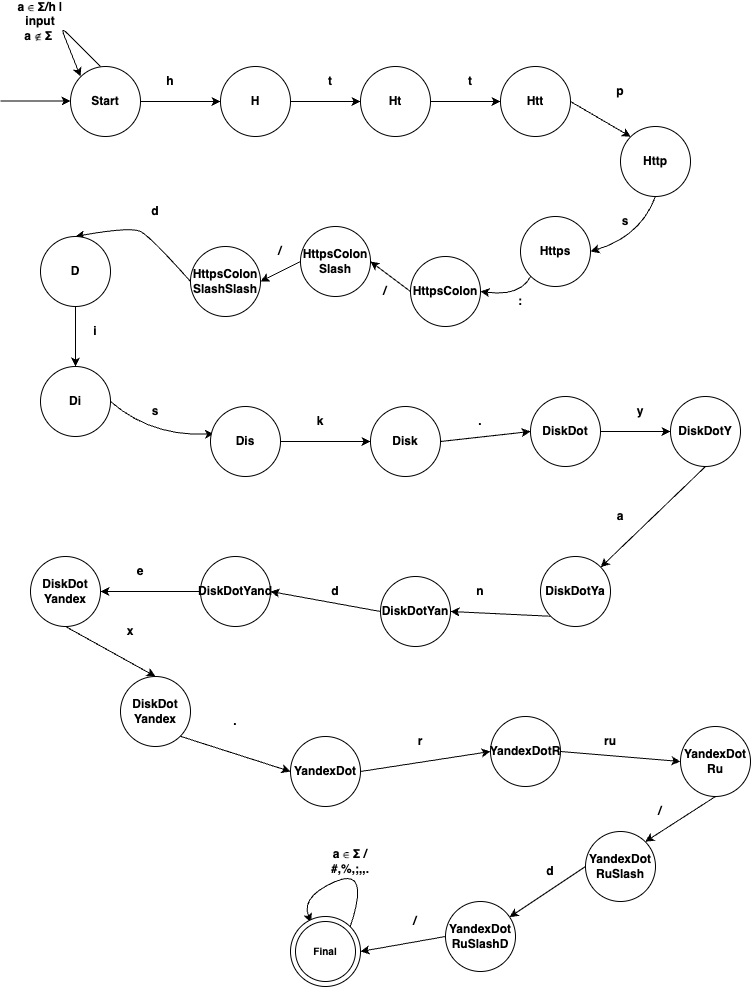
\includegraphics[width=0.9\textwidth]{NFA.png}
  \caption{Граф конечного автомата}
  \label{fig:DFA}
\end{figure}
\subsection{Граф ДКА}
\begin{figure}[H]
  \centering
  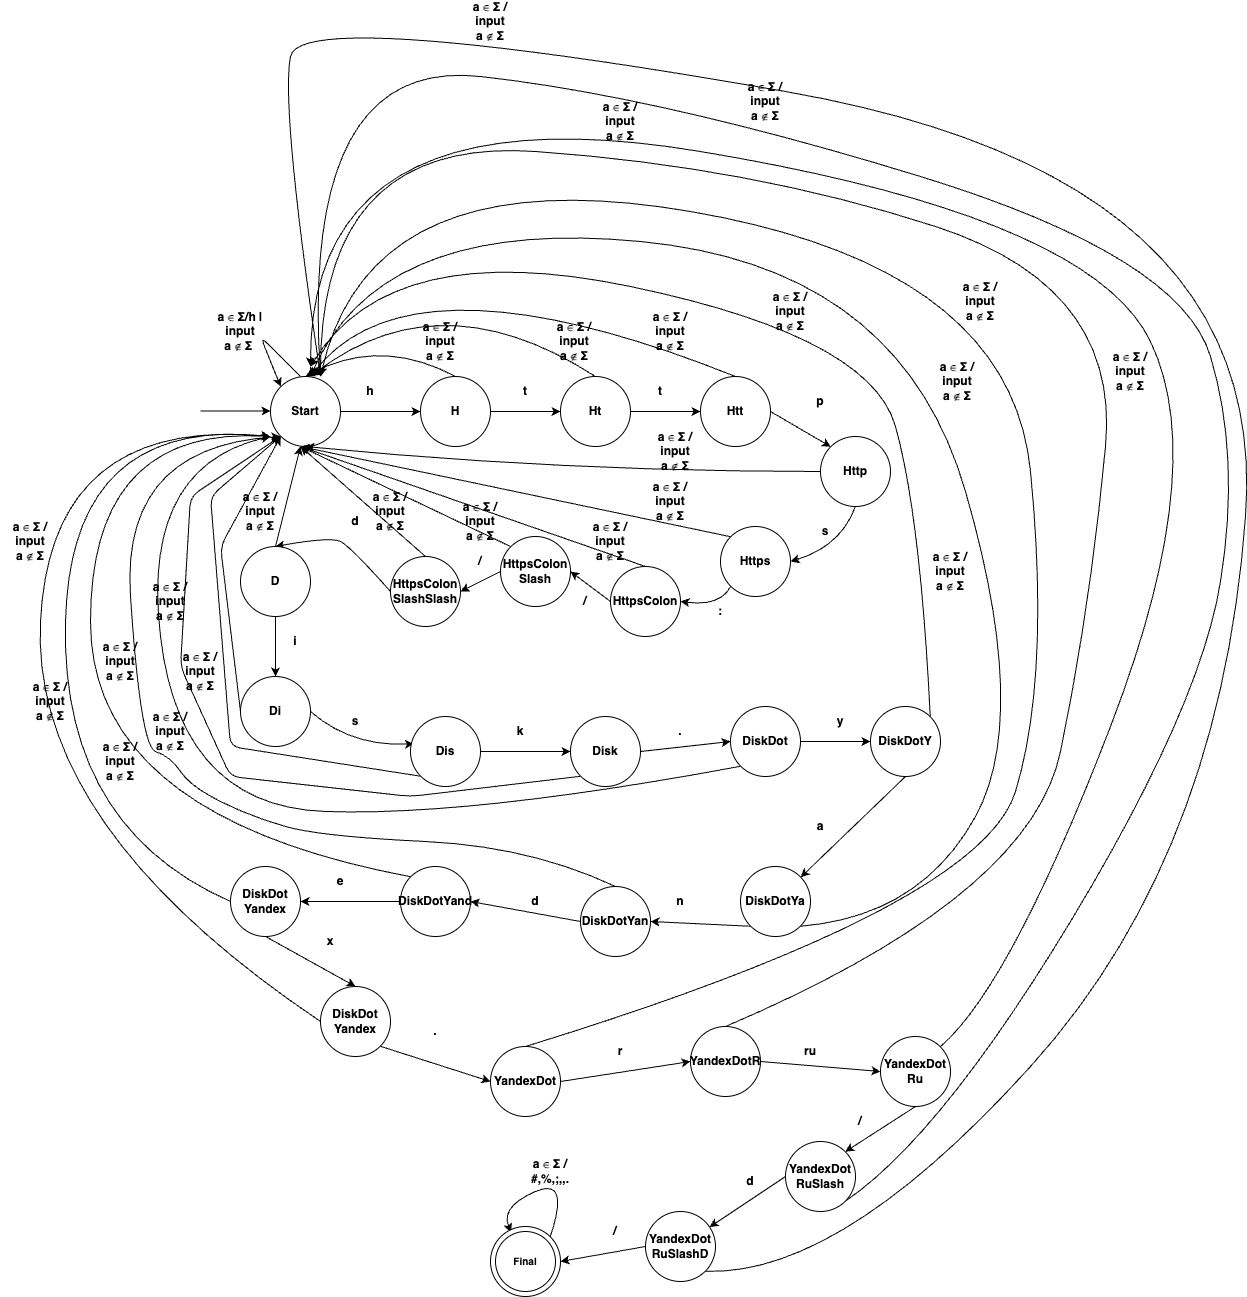
\includegraphics[width=1.0\textwidth]{DFA.png}
  \caption{Граф детерминированного конечного автомата}
  \label{fig:DFA}
\end{figure}
\newpage 
\section{Программная реализация}
В качестве языка программирования был выбран Haskell \\
В качестве стандарта языка, был выбран Haskell2010 \\
Для реализации программы, был собран cabal - проект, который включает в себя два .hs файла:
\begin{itemize}
	\item Lib.hs - Отвечающий за меню программы
	\item Main.hs - Отвечающий за управляющую логику
\end{itemize}
В листинге 1, представлен код Lib.hs. В листинге 2, представлен код Main.hs:
\subsection{Lib.hs}
Управляющая логика, основана на работе конечного автомата, на вход которого поступают введенные символы, далее функция переходов, переходи в следуюещее состояние, и так пока состояние не будет Final, либо пока не будет введен некорректный символ.
В качестве состояний автомата, был создан тип данных - State, а функции переходов transition определяются как State -> Char -> State. То есть: состояние, входной символ, следующее состояние. 
\begin{lstlisting}[caption={Lib.hs}, label={lst:example}]
	module Lib
    ( checkYandexDiskLink
    , generateValidLink
    ) where

import Data.Char (isAscii, isSpace, isControl)
import System.Random (randomRIO)
import Control.Monad (replicateM)
import Data.List (isInfixOf)

validChars :: String
validChars = ['a'..'z'] ++ ['0'..'9'] ++ "-_"

preprocess :: String -> String
preprocess = filter (not . isSpace) . map toLower
  where
    toLower c =
      if c >= 'A' && c <= 'Z'
      then toEnum (fromEnum c + 32)
      else c
      
data State = Start 
           | H | Ht | Htt | Https 
           | HttpsColon | HttpsColonSlash | HttpsColonSlashSlash
           | D | Di | Dis | Disk 
           | DiskDot | DiskDotY | DiskDotYa | DiskDotYan | DiskDotYand
           | DiskDotYande | DiskDotYandex 
           | YandexDot | YandexDotR | YandexDotRu 
           | YandexDotRuSlash
           | YandexDotRuSlashD 
           | YandexDotRuSlashDSlash
           | YandexDotRuSlashC
           | YandexDotRuSlashCl
           | YandexDotRuSlashCli
           | YandexDotRuSlashClie
           | YandexDotRuSlashClien
           | YandexDotRuSlashClient
           | YandexDotRuSlashClients
           | YandexDotRuSlashClientsSlash
           | YandexDotRuSlashClientsSlashD
           | YandexDotRuSlashClientsSlashDi
           | YandexDotRuSlashClientsSlashDis
           | YandexDotRuSlashClientsSlashDisk
           | YandexDotRuSlashClientsSlashDiskSlash
           | Y | Ya | Yad | Yadi
           | YadiDot | YadiDotS | YadiDotSk
           | YadiDotSkSlash
           | YadiDotSkSlashD
           | YadiDotSkSlashDSlash
           | Final
           deriving (Eq, Ord, Show, Enum, Bounded)

isValidChar :: Char -> Bool
isValidChar c = not (isSpace c || isControl c)

transition :: State -> Char -> State
transition Start 'h'                = H
transition H 't'                    = Ht
transition Ht 't'                   = Htt
transition Htt 'p'                  = Https
transition Https 's'                = HttpsColon
transition HttpsColon ':'           = HttpsColonSlash
transition HttpsColonSlash '/'      = HttpsColonSlashSlash
transition HttpsColonSlashSlash 'd' = D
transition HttpsColonSlashSlash 'y' = Y
transition Start 'd' = D
transition Start 'y' = Y
transition D 'i' = Di
transition Di 's' = Dis
transition Dis 'k' = Disk
transition Disk '.' = DiskDot
transition DiskDot 'y'      = DiskDotY
transition DiskDotY 'a'     = DiskDotYa
transition DiskDotYa 'n'    = DiskDotYan
transition DiskDotYan 'd'   = DiskDotYand
transition DiskDotYand 'e'  = DiskDotYande
transition DiskDotYande 'x' = DiskDotYandex
transition DiskDotYandex '.' = YandexDot
transition YandexDot 'r'       = YandexDotR
transition YandexDotR 'u'      = YandexDotRu
transition YandexDotRu '/' = YandexDotRuSlash
transition YandexDotRuSlash 'd' = YandexDotRuSlashD
transition YandexDotRuSlash 'c' = YandexDotRuSlashC    
transition YandexDotRuSlashD ' ' = YandexDotRuSlashD
transition YandexDotRuSlashD '/' = YandexDotRuSlashDSlash
transition YandexDotRuSlashDSlash _ = Final
transition YandexDotRuSlashC 'l' = YandexDotRuSlashCl
transition YandexDotRuSlashCl 'i' = YandexDotRuSlashCli
transition YandexDotRuSlashCli 'e' = YandexDotRuSlashClie
transition YandexDotRuSlashClie 'n' = YandexDotRuSlashClien
transition YandexDotRuSlashClien 't' = YandexDotRuSlashClient
transition YandexDotRuSlashClient 's' = YandexDotRuSlashClients
transition YandexDotRuSlashClients '/' = YandexDotRuSlashClientsSlash
transition YandexDotRuSlashClientsSlash 'd' = YandexDotRuSlashClientsSlashD
transition YandexDotRuSlashClientsSlashD 'i' = YandexDotRuSlashClientsSlashDi
transition YandexDotRuSlashClientsSlashDi 's' = YandexDotRuSlashClientsSlashDis
transition YandexDotRuSlashClientsSlashDis 'k' = YandexDotRuSlashClientsSlashDisk
transition YandexDotRuSlashClientsSlashDisk '/' = YandexDotRuSlashClientsSlashDiskSlash
transition YandexDotRuSlashClientsSlashDiskSlash _ = Final
transition Y 'a'     = Ya
transition Ya 'd'    = Yad
transition Yad 'i'   = Yadi
transition Yadi '.'  = YadiDot
transition YadiDot 's' = YadiDotS
transition YadiDotS 'k' = YadiDotSk
transition YadiDotSk '/' = YadiDotSkSlash
transition YadiDotSkSlash 'd' = YadiDotSkSlashD
transition YadiDotSkSlashD '/' = YadiDotSkSlashDSlash
transition YadiDotSkSlashDSlash _ = Final

transition Final c
    | isValidChar c = Final
    | otherwise     = Start
transition s ' '
    | s /= Final  = s
    | otherwise   = Final
transition _ _ = Start

checkYandexDiskLink :: String -> IO ()
checkYandexDiskLink input = do
    if not (all isAscii input)
        then putStrLn "Oops! Only ASCII symbols!"
        else do
            let processed = preprocess input
            if isMainPage processed
                then putStrLn "Yandex Disk main page"
                else do
                    let result = processString processed Start
                    if result == Final && hasValidPath processed
                        then putStrLn "String - is a Yandex Disk link"
                        else putStrLn "Oops! Not a Yandex Disk link"
  where
    isMainPage :: String -> Bool
    isMainPage s = 
        let normalized = preprocess s
        in  normalized == "https://disk.yandex.ru"
         || normalized == "disk.yandex.ru"
         || normalized == "https://disk.yandex.ru/"
         || normalized == "disk.yandex.ru/"
         || normalized == "disk.yandex.ru/clients/"
         || normalized == "disk.yandex.ru/clients/disk/"
         || normalized == "yadi.sk"
         || normalized == "yadi.sk/"

    processString :: String -> State -> State
    processString [] st     = st
    processString (c:cs) st = processString cs (transition st c)
    
    hasValidPath :: String -> Bool
    hasValidPath s
      | "disk.yandex.ru/d/" `isInfixOf` s = True
      | "disk.yandex.ru/clients/disk/" `isInfixOf` s = True
      | "yadi.sk/d/" `isInfixOf` s = True
      | otherwise = False

generateValidLink :: IO String
generateValidLink = do
    idLength <- randomRIO (12, 20)
    idPart   <- replicateM idLength (randomChar validChars)
    patternIndex <- randomRIO (1 :: Int, 3)
    return $ case patternIndex of
        1 -> "https://disk.yandex.ru/d/" ++ idPart
        2 -> "https://disk.yandex.ru/clients/disk/" ++ idPart
        3 -> "https://yadi.sk/d/" ++ idPart
        _ -> "https://disk.yandex.ru/d/" ++ idPart
  where
    randomChar :: String -> IO Char
    randomChar chars = do
        idx <- randomRIO (0, length chars - 1)
        return (chars !! idx)
\end{lstlisting}
\textbf{Функция preprocess}
\begin{itemize}
  \item Тип: \texttt{String -> String}
  \item На входе: строка исходного текста (например, введённая ссылка)
  \item На выходе: строка без пробелов (и приведённая к нижнему регистру)
  \item Нужна для: очистки входной строки перед проверкой или генерацией ссылки
\end{itemize}

\textbf{Функция checkYandexDiskLink}
\begin{itemize}
  \item Тип: \texttt{String -> IO ()}
  \item На входе: строка, содержащая ссылку
  \item На выходе: IO-экшн, который выводит сообщение о результате проверки
  \item Нужна для: проверки, является ли введённая строка валидной ссылкой Яндекс Диска
\end{itemize}

\textbf{Функция generateValidLink}
\begin{itemize}
  \item Тип: \texttt{IO String}
  \item На входе: отсутствует (генерируется случайным образом)
  \item На выходе: сгенерированная строка, представляющая валидную ссылку Яндекс Диска
  \item Нужна для: автоматической генерации валидных ссылок
\end{itemize}

\textbf{Функция transition}
\begin{itemize}
  \item Тип: \texttt{State -> Char -> State}
  \item На входе: текущее состояние автомата и входной символ (\texttt{Char})
  \item На выходе: новое состояние автомата
  \item Нужна для: реализации функции переходов конечного автомата, определяющей, в какое состояние перейти для данного символа
\end{itemize}

\textbf{Функция processString}
\begin{itemize}
  \item Тип: \texttt{String -> State -> State}
  \item На входе: строка для обработки и начальное состояние автомата
  \item На выходе: конечное состояние автомата после обработки всей строки
  \item Нужна для: последовательного применения функции \texttt{transition} ко всем символам входной строки
\end{itemize}
\subsection{Main.hs}
\begin{lstlisting}[caption={Main.hs}, label={lst:example}]
module Main where
import Lib
	
	main :: IO ()
	main = do
		putStrLn "Select an option:"
		putStrLn ""
		putStrLn "1. Check the link"
		putStrLn ""
		putStrLn "2. Generate a valid link"
		putStrLn ""
		putStrLn "3. Show link pattern"
		putStrLn ""
		putStrLn "4. Exit"
		putStrLn ""
		putStrLn "Enter the number and press Enter:"
		choice <- getLine
	
		case choice of
			"1" -> do
				putStrLn ""
				putStrLn "Enter the link to check:"
				putStrLn ""
				input <- getLine
				checkYandexDiskLink input
				main
			"2" -> do
				putStrLn ""
				link <- generateValidLink
				putStrLn $ "Generated link: " ++ link
				putStrLn ""
				main
			"3" -> do
				putStrLn ""
				putStrLn $ "Pattern /d/: " ++ "https://disk.yandex.ru/d/..."
				putStrLn $ "Pattern /clients/: " ++ "https://yadi.sk/d/..."
				putStrLn $ "Pattern /clients/disk/: " ++ "https://disk.yandex.ru/clients/disk/..."
				putStrLn ""
				main
			"4" -> putStrLn "Goodbye!"
			_ -> do
				putStrLn ""
				putStrLn ""
				putStrLn "Invalid choice, please try again"
				putStrLn ""
				putStrLn ""
				main
\end{lstlisting}
\begin{itemize}
	\item Монада IO, выводит меню
	\item Обертка do, вызывает кейс для выбора подпрограмм программы, где:
	\begin {enumerate}
	\item Проверка строки на соответствие ссылки Яндекс Диска
	\subitem Вызывает функцию checkYandexDiskLink
	\item Генератор валидной ссылки Яндекс Диска
	\subitem Вызывает функцию generateValidLink и перечисляет его в лист
	\item Демонстрация шаблонов
	\subitem Выводит шаблоны в консоль среды разработки
	\item Завершение программы
	\subitem Завершает программу и выводит сообщение
	\end{enumerate}
\end{itemize}
При ином входе в main функцию, выводится сообщение о неверном выборе, затем происходит возврат в меню.

\newpage
\section*{Заключение}
\addcontentsline{toc}{section}{Заключение}
В результате выполнения лабораторной работы, был реализован cabal-проект, содержащий код программы, работающий на логике конечного автомата, который проверяет регулярное выражение - ссылку на Яндекс Диск. 
Были реализованы три варианта обращения к сайту:
\begin{itemize}
	\item https://disk.yandex.ru/d/\dots
	\item https://disk.yandex.clients/d/\dots
	\item https://yadisk.ru/d/\dots
\end{itemize}
\emph{Плюсы}:
\begin{itemize}
	\item ДКА обрабатывает входную строку за линейное время относительно её длины.
	\item Язык Haskell, позволяет реализовать переходы в ДКА, как чистые функции. Позволяет избежать побочных эффектов.
	\item Была реализована функция преведения ссылки в нормальную форму (без пробелов).
\end{itemize}
\emph{Минусы}:
\begin{itemize}
	\item Большое количество состояний и переходов сказывается на скорости работы программы.
	\item Любое изменение формата ссылки требует правок во многих правилах переходов, что увеличивает риск ошибок.
	\item Отсутствие явного логгирования.
\end{itemize}
\emph{Масштабируемость}:
\begin{itemize}
	\item Добавить явный вывод ошибок в входной строке.
	\item Реализация проверок иных сайтов Яндекса.
	\item Разбиение обработок на модули для разных ссылок.
\end{itemize}
\newpage
\section*{Список литературы}
\addcontentsline{toc}{section}{Список литературы}
\begin{enumerate}
    \item \begin{sloppypar}Востров, А. В. Математическая логика [Электронный ресурс]. Режим доступа: https://tema.spbstu.ru/compiler/ (последний визит: 01.04.2025). \end{sloppypar}
    \item Сети, Р.; Ахо, А. Компиляторы: принципы, технологии и инструменты / Р. Сети, А. Ахо. – М.: Издательство «Наука», 2006. – С. 104.
\end{enumerate}
\end{document}
